\documentclass[10pt,twocolumn,letterpaper]{article}

\usepackage{cvpr}
\usepackage{times}
\usepackage{epsfig}
\usepackage{graphicx}
\usepackage{amsmath}
\usepackage{amssymb}

% Include other packages here, before hyperref.

% If you comment hyperref and then uncomment it, you should delete
% egpaper.aux before re-running latex.  (Or just hit 'q' on the first latex
% run, let it finish, and you should be clear).
\usepackage[breaklinks=true,bookmarks=false]{hyperref}

\cvprfinalcopy % *** Uncomment this line for the final submission

\def\cvprPaperID{****} % *** Enter the CVPR Paper ID here
\def\httilde{\mbox{\tt\raisebox{-.5ex}{\symbol{126}}}}

% Pages are numbered in submission mode, and unnumbered in camera-ready
%\ifcvprfinal\pagestyle{empty}\fi
\setcounter{page}{4321}
\begin{document}

%%%%%%%%% TITLE
\title{\LaTeX\ Author Guidelines for CVPR Proceedings}

\author{First Author\\
Institution1\\
Institution1 address\\
{\tt\small firstauthor@i1.org}
% For a paper whose authors are all at the same institution,
% omit the following lines up until the closing ``}''.
% Additional authors and addresses can be added with ``\and'',
% just like the second author.
% To save space, use either the email address or home page, not both
\and
Second Author\\
Institution2\\
First line of institution2 address\\
{\tt\small secondauthor@i2.org}
}

\maketitle
%\thispagestyle{empty}

%%%%%%%%% ABSTRACT
\begin{abstract}
   The ABSTRACT is to be in fully-justified italicized text, at the top
   of the left-hand column, below the author and affiliation
   information. Use the word ``Abstract'' as the title, in 12-point
   Times, boldface type, centered relative to the column, initially
   capitalized. The abstract is to be in 10-point, single-spaced type.
   Leave two blank lines after the Abstract, then begin the main text.
   Look at previous CVPR abstracts to get a feel for style and length.
\end{abstract}

%%%%%%%%% BODY TEXT
\section{Introduction}
	Reconstructing a 3D object from input images is an essential task in the field of computer vision. Recent advances in photo databases have led to an increase in the use of 3D reconstruction. While there have been many recent advances in 3D reconstruction, most new techniques still suffer from the same problems which plagued original methods. 
First, many approaches require a camera calibration for each image used in the 3D reconstruction. This calibration is necessary to obtain the intrinsic and extrinsic parameters of the camera which are used to project points from 2D images into 3D space. Performing calibrations for each image is impractical for new approaches that emphasize using as many images as possible for the reconstruction.
	The other setback relates to user input. Many approaches require users to pick points on the input images that specify either the object to reconstruct or the planes used to perform the reconstruction. While user input may improve the reconstruction as it improves depth detection and crops the image so only necessary points are used, it does not encourage using many input images. Several techniques overcome these setbacks by performing reconstruction based on uncalibrated images obtained by the same, freely moving camera. Camera calibration must be performed once and the resulting parameters can be used for the reconstruction across all input images. 
	Capturing pairs of feature points from the input images is an important step in the 3D reconstruction process. There are several feature point detection algorithms which are currently used by many reconstruction techniques, though each has its own setbacks. Two popular approaches are Scale Invariant Feature Transform (SIFT) and corner extraction algorithms such as Harris corner detection. Each approach yields pairs of matched feature points across the input images. 
	In this paper, we develop a new technique which reconstructs a 3D object from two input images captured by a freely moving camera. We then combine SIFT and Harris corner detection to obtain the relevant pairs of feature points from the two input images. Prior to using these matching points, we use the Random Sample Consensus (RANSAC) algorithm to remove outlier matches. We calculate the intrinsic parameters of the camera used to take the input images with Zhang’s method. Using the intrinsic parameters of the camera and the matched feature points from the input images, we are able to obtain a 3D reconstruction for the primary object in the image. 
\section{Introduction}
\label{s:intro}

Reconstructing a 3D object from multiple input images is an essential task in the field of computer vision. Recent advances in photo databases have led to an increase in the use of 3D reconstruction. While there have been many recent advances in 3D reconstruction, most new techniques still suffer from the same problems which plagued original methods. 

First, many approaches require a camera calibration for each image used in the 3D reconstruction. This calibration is necessary to obtain the intrinsic and extrinsic parameters of the camera which are used to project points from 2D images into 3D space. Performing calibrations for each image is impractical for new approaches that emphasize using as many images as possible for the reconstruction.

The other setback relates to user input. Many approaches require users to pick points on the input images that specify either the object to reconstruct or the planes used to perform the reconstruction. While user input may improve the reconstruction as it improves depth detection and crops the image so only necessary points are used, it does not encourage using many input images. Several techniques overcome these setbacks by performing reconstruction based on uncalibrated images obtained by the same, freely moving camera. Camera calibration is performed once and the resulting parameters are used for the reconstruction across all input images. 

Capturing pairs of feature points from the input images is an important step in the 3D reconstruction process. There are several feature point detection algorithms which are currently used by many reconstruction techniques, though each has its own setbacks. Two popular approaches are Scale Invariant Feature Transform (SIFT) and corner extraction algorithms such as Harris corner detection. Each approach yields pairs of matched feature points across the input images. 

In this project, we develop a new technique which reconstructs a 3D object from two input images captured by a freely moving camera. We combine SIFT and Harris corner detection to obtain the relevant pairs of feature points from the two input images. Prior to using these matched feature points, we use the Random Sample Consensus (RANSAC) algorithm to remove outlier matches. We calculate the intrinsic parameters of the camera used to take the input images with Zhang’s method. Using the intrinsic parameters of the camera and the matched feature points from the input images, we are able to obtain a 3D reconstruction for the primary object in the image.

The report is organized as follows. Section~\ref{s:related} describes related work, and then section~\ref{s:overview} provides an overview of our algorithm. Then, the later sections delve into more details. Section~\ref{s:camera} and~\ref{s:sift} discuss camera calibration and automated feature detection which are tools that we use in our reconstruction. Section~\ref{s:fundamental} describes the relevant epipolar geometry, and section~\ref{s:reconstruction} explains how to use the epipolar geometry to do the 3D reconstruction. We show some results in section~\ref{s:results}. We talk about our individual contributions in section~\ref{s:contribution}, and we conclude in section~\ref{s:conclusion}.


\section{Related Work}
\section{Related Work}
\label{s:related}
There has been much work on reconstructing 3D object from multiple images using epipolar geometry. A good review of the methods and previous work in this area can be found here~\cite{epipolar_review}. Our project uses many of these techniques and combines them with more modern automation techniques, such as SIFT and Harris corners to reduce the amount of human interaction required for the reconstruction. Our technique is primarily based on the work of Peng et al.~\cite{SIFT/Harris}, who use these automated techniques and enhancements to perform the 3D reconstruction.

There is also a separate set of work that tries to do 3D reconstruction using only a single uncalibrated image~\cite{single_image, single_image2}. However, these type of reconstructions either require some prior knowledge about the parameters of the scene and the camera, or significant user input throughout the reconstruction process. Multiple view 3D reconstruction does not require any prior knowledge because we can extract the necessary parameters from the images.

\section{Overview}
In this section, we give an overview of our algorithm, and in later sections,
we describe the different components in more details.
\section{Overview}
\label{s:overview}

In this section, we give an overview of our algorithm, which we will describe in more detail
in later sections.

\begin{enumerate}
\item{We find the intrinsic parameters of our camera using Zhang's method.}
\item{Using SIFT and Harris corner detection, we identify pairs of features points on both images, and we use RANSAC to find the inliers so that we can generate a representative fundamental matrix.}
\item{With the intrinsic parameters of our camera and the fundamental matrix, we can derive the essential matrix.}
\item{The essential matrix is used to derive the projection matrices of the images which each comprise of a rotation matrix and translation vector. With this information, we can reconstruct the 3d image using triangulation.}
\end{enumerate}


\section{Camera Calibration}
We use a pinhole camera model. Here, we obtain the intrinsic parameters
using Zhang's method.
\section{Camera Calibration}
\label{s:camera}

To calibrate our camera and obtain its intrinsic parameters, we use Zhang's method. 
Zhang's method is a technique that uses several images to derive a camera’s focal length, aspect ratio, and principal points. While there are many other approaches to performing this essential task, Zhang's method is the best tradeoff between flexiblity and robustness. The two traditional approaches are often categorized as either photogrammetric or self-calibration. Photogrammetric methods require using a 3D object whose 3D coordinates are precisely known. Taking multiple images of this 3D object lets one infer the intrinsic parameters of the camera as they can be derived from the difference between the actual coordinates of the object and what is seen across the images. However, the apparatus necessary to perform this type of calibration is expensive. Self-calibration, while less costly, is not reliable as there are often not enough known points to estimate all the necessary parameters. Self-calibration requires moving the camera in a static setup and performing a feature points matching across the considered images. For each used image, self-calibration methods infer constraints pertaining to the rigidity of the object considered. Collectively, these constraints ultimately lead to a valid set of intrinsic parameters. 

Zhang's method is a cross between photogrammetric and self-calibration techniques. Zhang's method requires one to construct a pattern on a paper and attach it to a planar surface. Several images of the pattern, from different angles, are then taken. As long as the camera or the pattern is stationary, the movement is not restricted. Using an understanding of the geometry of the designed pattern, constraints on the intrinsic parameters arise from each view. Using all of these constraints, a set of intrinsic parameters which satisfy all the considered views can be inferred. Of course, using more views will yield intrinsic parameters closer to their actual values. Thus, Zhang’s method incorporates understanding 3D coordinates of the pattern  (photogrammetric) and using multiple views to set constraints on the intrinsic parameters (self-calibration), but it only considers one plane and a user-designed pattern. In their paper, Zhang et. al. show that their calibration technique is both flexible, robust, and accurate. 

A camera's intrinsic matrix is defined as:\\
\[
   A =
  \left[ {\begin{array}{ccc}
   \alpha & \gamma & u0  \\
   0 & \beta & v0 \\
   0 & 0 & 1 \\
  \end{array} } \right]
\] \\
where (u0, v0) is the principal point, $\alpha$ and $\beta$ are image scale factors, and $\gamma$ is a parameter which describes the skew in the image axes. We use the pinhole camera model which dictates that a 3D point, M, is related to its image projection, m, by:
\begin{equation}
  sm = A
  \left[ {\begin{array}{cc}
   R & t \\
  \end{array} } \right]
  M \\
\end{equation}
where R is the rotation matrix and t is the translation vector of the considered image. 
For each view used, we estimate a homography matrix:
\begin{equation}
  H =
  \left[ {\begin{array}{ccc}
   h_1 & h_2 & h_3 \\
  \end{array} } \right]
  = \lambda  A
  \left[ {\begin{array}{ccc}
   r_1 & r_2 & t \\
  \end{array} } \right]
  \\
\end{equation}
where $r_1$ and $r_2$ are the components of the rotation matrix, R, and lambda is a scaling factor.  Since $r_1$ and $r_2$ are orthonormal, we can derive the following two constraints:
\begin{equation}
  h_1^T A^{-T} A^{-1} h_2 = 0
\end{equation}
\begin{equation}
  h_1^T A^{-T} A^{-1} h_1 = h_2^T A^{-T} A^{-1} h_2
\end{equation}

The approximation of the camera's intrinsic parameters is improved using a maximum-likelihood estimation. Zhang's method also extracts the camera's extrinsic parameters for the given input images, but we do not make use of this data as we are reconstructing an object separate from the considered planar pattern. 


\section{Fundamental and Essential Matrix}
The fundamental matrix contains information about the intrinsic and extrinsic parameters
of the camera. 
\section{Geometry of 3D Reconstruction}
\label{s:fundamental}
In order to understand the purpose of the fundamental and essential matrix, we first describe epipolar geometry. Epipolar geometry captures the intrinsic projective geometry between two cameras views, which only depends on the internal parameters of the camera and relative positions of the two views. The fundamental matrix contains this information, and from the fundamental matrix, we can derive the essential matrix, which gives us the relative position and orientation of the two camera views. From that, we can derive the actual 3d points of the points in both views.

\subsection{Epipolar Geometry}
In our project, we take two uncalibrated pictures of the same object but from different views. Epipolar geometry gives us a relationship between these images.
\begin{figure}[H]
\begin{center}
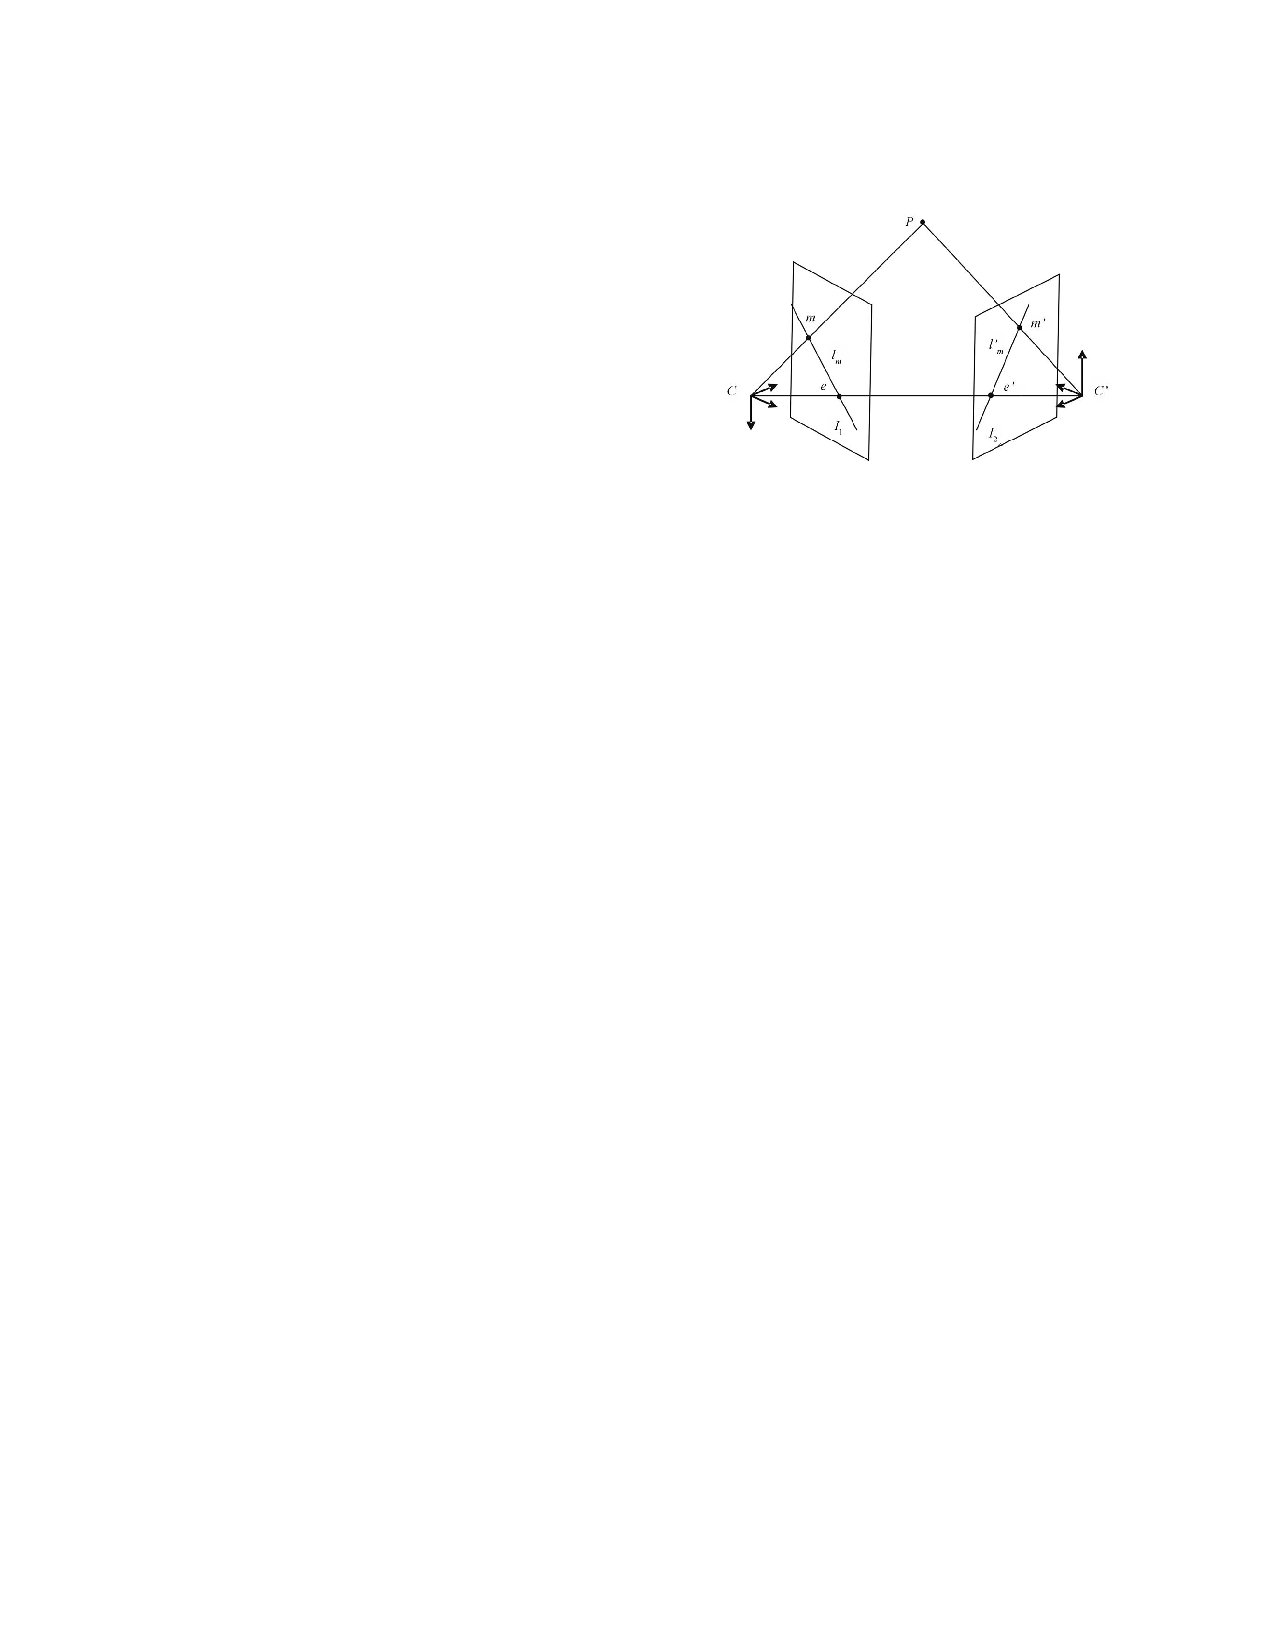
\includegraphics[width=0.9\linewidth]{figures/epipolar.pdf}
\end{center}
\caption{Epipolar geometry of two images from different views.}
\label{epipolar_pic}
\end{figure}

Figure~\ref{epipolar_pic} illustrates the relevant epipolar geometry. $I_1$ and $I_2$ are the images planes and $C$ and $C'$ represent the optical center of the camera from different views. $m$ and $m'$ represent $P$ projected onto $I_1$ and $I_2$ respectively. $e$ and $e'$ represent the epipoles, which are the intersections of the image planes with the line connects the camera centers. $l_m$ and $l_m'$ are the epipolar lines, which is where the epipolar plane intersects the image plane. It is important to note that $m$ and $m'$ lie on the $l_m$ and $l_m'$ respectively. As a result, we know that the matching point for $m$ is going to be on the line $l_m'$ in $I_2$ instead of anywhere in space of $I_2$. In order to capture this geometric restriction, we use the fundamental matrix, which will describe in the next section.

\subsection{Fundamental Matrix}
The fundamental matrix $F$ is a mathematical representation of the epipolar geometry described above. From Figure~\ref{epipolar_pic}, we can see that for a point $m$ in $I_1$, there is a corresponding epipolar line $l_m'$ in $I_2$ and the matching point $m'$ must lie on that line. We can think of this as a mapping from a point to a line, specifically a projective mapping from points to lines. This projection is represented by the fundamental $F$. Algebraically, two matching points $m$ and $m'$ on two images must satisfy the following relation:
\begin{equation}
m^TFm = 0
\end{equation}

There are many methods to find the fundamental matrix for a specific pair of images algebraically and geometrically. Each method has its tradeoffs for time, complexity, and error. For the sake of space, we provide a high level overview of how we calculated the fundamental matrix as many of the details vary based on implementation. The fundamental matrix is a 3x3 matrix, so there are 9 parameters. However, after normalizing on one parameter, we only need to find 8 parameters. This means we need at least 8 pairs of points to construct the matrix. To obtain points for corresponding features in the two images, we used SIFT~\ref{sift}, which will be described later in the paper, but there are also many other ways to obtains these points. However, in most of these methods, we have many more than 8 points. We use RANSAC~\cite{ransac} to filter out outliers and calculate $F$ such that there are the largest number of inliers. To calculate the fundamental matrix, we use the least median squares method~\cite{lms_zhang} to minimize error. 

We now want to obtain the extrinsic parameters (orientation and translation) from the fundamental matrix, which are found in the essential matrix.

\subsection{Essential Matrix}
The essential matrix gives us the extrinsic parameters of the two views. In other words, we can find the translation and rotation of the views relative to each other. However, we can only use the essential matrix if we know the internal parameters of the camera. In section~\ref{s:calibration}, we describe a method to find the internal parameters of the camera. With that, we have the following relation between essential matrix and fundamental matrix:
\begin{equation}
E = K^TFK
\end{equation}
$F$ is the fundamental matrix and $K$ is the internal parameters of the camera.

Theoretically, the essential matrix should have two equal non-zero eigenvalues and a zero eigenvalue. However, due to the noise in the data, this usually is not true in practice. In order to rectify this, we use Singular Value Decomposition (SVD)~\cite{svd} to capture the diagonal matrix with the eigenvalues. We set the smallest eigenvalue to 0 and set the other two eigenvalues as the average of each other. Then, with this diagonal matrix, we construct a new essential matrix.

Now, we have all the tools to perform the 3D reconstruction.


\section{3D reconstruction}
We use the fundamental and essential matrix to reconstruct the 3d image.
\section{3D Reconstruction}
\label{s:reconstruction}
Having all the necessary tools, we now reconstruct the 3D image. First, we describe the perspective projective transform from 3D to 2D using the projective matrix $P$. It is important to note that we use the pinhole camera model. Let $m$ be the 2D image point in homogeneous coordinates and $M$ be the point in 3D space in homogeneous coordinates. We use the projective matrix $P$ to related $m$ and $M$.
\begin{equation}
m = PM = K[R | t]M
\end{equation}
where $K$ is the intrinsic parameters of the camera, $R$ is the rotation matrix, and $t$ is the translation matrix.

We now need to create the projective matrices for each image. For simplicity, we set the first image to be the world coordinates, so our projective matrix is defined as:
\begin{equation}
P_1 = K[I | 0] = [K | 0]
\end{equation}

Now, we need to find the projective matrix for the second image $P_2$ relative to the world coordinates represented by $P_1$. More specifically, we need to find the rotation and translation matrix for this image, with respect to the first image. Since we calibrated the camera using Zhang's method, this can be done using the essential matrix. We take the SVD of the essential matrix $E$ to decompose it and we assume the following $W$:
\begin{equation*}
E = USV^T, \; \text{suppose} \; W =
  \left[ {\begin{array}{ccc}
   0 & -1 & 0  \\
  1 & 0 & 0 \\
   0 & 0 & 1 \\
  \end{array} } \right]
\end{equation*}

There are two possible values for the rotation matrix: $R=UWV^T$ or $R=UW^TV^T$. There are also two possible values for the translation vector: $t = u_3$ or $t=-u_3$ where $u_3$ is the last column of $U$. Since $P_2 = K[R |t]$, we have four possible values for $P_2$. In order to pick the correct one, we calculate the 3D spatial coordinate for one pair of matching features. We then pick the $P_2$ such that the point is in front of both cameras. In our case, this means that the Z coordinate of the 3D coordinate is positive. 

After we have the projective matrix for each image, we calculate the 3D spatial point $M = (X, Y, Z, 1)$ for each set of matching points $m = (u_1, v_1, 1)$ and $m' = (u_2, v_2, 1)$. Suppose $P_{1i}$ and $P_{2i}$ are the $i$th row vector of $P_1$ and $P_2$ respectively. To obtain the 3D spatial coordinate $M$, we have the following equation to perform triangulation for each $m$, $m'$ pair:
\begin{equation*}
  \left[ {\begin{array}{c}
   P_{13}u_1 - P_{11} \\
   P_{13}v_1 - P_{12} \\
   P_{23}u_2 - P_{21} \\
   P_{23}v_2 - P_{22} \\
  \end{array} } \right] M = 0
\end{equation*}

We can use the least square method to find $M$ for each pair of matching points. Once we have all the 3D spatial points, we can reconstruct the image.

\section{Results}
Here we show some of our reconstructions. We used a camera with the following intrinsic
parameters.
\section{Results}
\label{s:results}

Here, we show some of our reconstructions as well as illustrate the implementation of our immediate steps, such as the SIFT matching points and Zhang's method. We used a Panasonic Lumix DMC-ZS5 camera to take pictures.

\subsection{Camera Calibration}
As stated above, we use Zhang's method to calibrate our camera. We use a sheet of paper with six 2" by 2" black boxes. Some pictures of the different angles used for the calibration are shown in Figure~\ref{calib_pics}. 

\begin{figure}[H]
\begin{center}
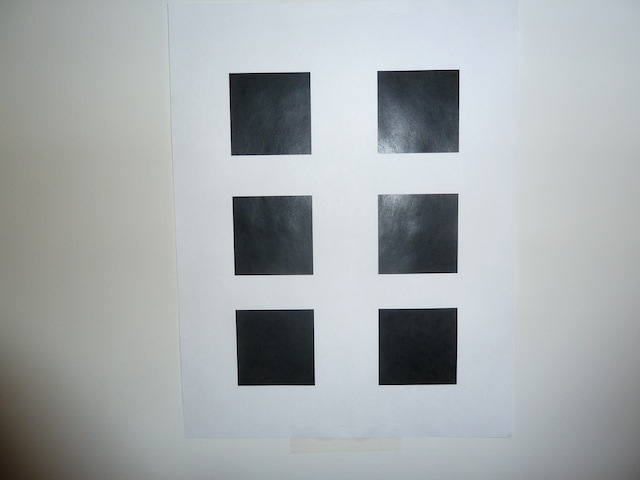
\includegraphics[width=0.45\linewidth]{figures/calib1.jpg}
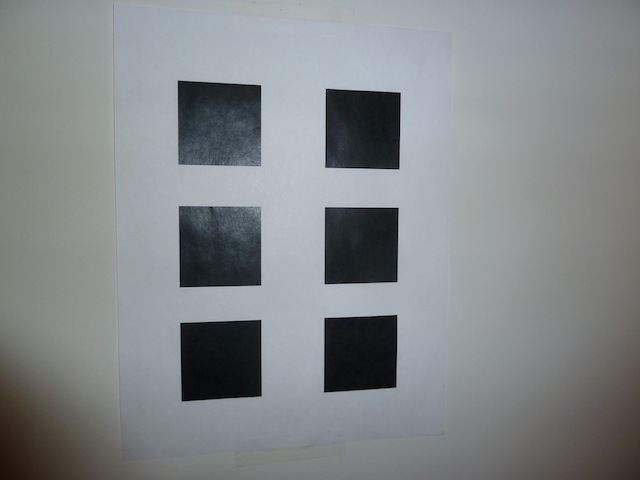
\includegraphics[width=0.45\linewidth]{figures/calib2.jpg}
\end{center}
\caption{Different calibration angles for Zhang's method}
\label{calib_pics}
\end{figure}

We used multiple views and took the average over different permutations. We found the following intrinsic parameter matrix $K$ for this camera:
\begin{equation*}
K =
  \left[ {\begin{array}{ccc}
   360.506 & -38.7974 & 128.692  \\
  0 & 470.953 & 162.864 \\
   0 & 0 & 1 \\
  \end{array} } \right]
\end{equation*}

\subsection{Reconstruction of Zhang's images}
We first reconstructed the images provided by Zhang~\cite{Calibration} because we were provided with the pictures and internal parameters. 

\section{Conclusion}
\label{s:conclusion}
This project describes a flexible and practical 3D-reconstruction technique. Rather than having to perform a camera calibration for each input image used in the reconstruction, as many previous techniques have required, we only perform the calibration once using Zhang’s method. Thus, this approach scales well with the number of input images used, as long as they are all taken with the same camera. We also combine several common feature point extraction methods to enhance the detail in the final 3D reconstruction. Using both SIFT and Harris corner detection, we are able to get enough pairs of matching points to recover all eight unknowns in the fundamental matrix while incorporating all the necessary feature points to capture depth and structural details in the reconstructed object. The benefits of including Harris corner detection are highlighted in the results we provided. Both edges and corners are much more pronounced in the reconstructed images using corner detection than in those when we used SIFT alone. 



\begin{figure}[t]
\begin{center}
\fbox{\rule{0pt}{2in} \rule{0.9\linewidth}{0pt}}
   %\includegraphics[width=0.8\linewidth]{egfigure.eps}
\end{center}
   \caption{Example of caption.  It is set in Roman so that mathematics
   (always set in Roman: $B \sin A = A \sin B$) may be included without an
   ugly clash.}
\label{fig:long}
\label{fig:onecol}
\end{figure}

\subsection{Miscellaneous}

\noindent
Compare the following:\\
\begin{tabular}{ll}
 \verb'$conf_a$' &  $conf_a$ \\
 \verb'$\mathit{conf}_a$' & $\mathit{conf}_a$
\end{tabular}\\
See The \TeX book, p165.

The space after \eg, meaning ``for example'', should not be a
sentence-ending space. So \eg is correct, {\em e.g.} is not.  The provided
\verb'\eg' macro takes care of this.

When citing a multi-author paper, you may save space by using ``et alia'',
shortened to ``\etal'' (not ``{\em et.\ al.}'' as ``{\em et}'' is a complete word.)
However, use it only when there are three or more authors.  Thus, the
following is correct: ``
   Frobnication has been trendy lately.
   It was introduced by Alpher~\cite{Alpher02}, and subsequently developed by
   Alpher and Fotheringham-Smythe~\cite{Alpher03}, and Alpher \etal~\cite{Alpher04}.''

This is incorrect: ``... subsequently developed by Alpher \etal~\cite{Alpher03} ...''
because reference~\cite{Alpher03} has just two authors.  If you use the
\verb'\etal' macro provided, then you need not worry about double periods
when used at the end of a sentence as in Alpher \etal.

For this citation style, keep multiple citations in numerical (not
chronological) order, so prefer \cite{Alpher03,Alpher02,Authors13} to
\cite{Alpher02,Alpher03,Authors13}.


\begin{figure*}
\begin{center}
\fbox{\rule{0pt}{2in} \rule{.9\linewidth}{0pt}}
\end{center}
   \caption{Example of a short caption, which should be centered.}
\label{fig:short}
\end{figure*}

%-------------------------------------------------------------------------
\subsection{Margins and page numbering}

All printed material, including text, illustrations, and charts, must be kept
within a print area 6-7/8 inches (17.5 cm) wide by 8-7/8 inches (22.54 cm)
high.
Page numbers should be in footer with page numbers, centered and .75
inches from the bottom of the page and make it start at the correct page
number rather than the 4321 in the example.  To do this fine the line (around
line 23)  
\begin{verbatim}
%\ifcvprfinal\pagestyle{empty}\fi
\setcounter{page}{4321}
\end{verbatim}
where the number 4321 is your assigned starting page.  

Make sure the first page is numbered by commenting out the first page being
empty on line 46
\begin{verbatim}
%\thispagestyle{empty}
\end{verbatim}


%-------------------------------------------------------------------------
\subsection{References}

List and number all bibliographical references in 9-point Times,
single-spaced, at the end of your paper. When referenced in the text,
enclose the citation number in square brackets, for
example~\cite{Authors13}.  Where appropriate, include the name(s) of
editors of referenced books.

\begin{table}
\begin{center}
\begin{tabular}{|l|c|}
\hline
Method & Frobnability \\
\hline\hline
Theirs & Frumpy \\
Yours & Frobbly \\
Ours & Makes one's heart Frob\\
\hline
\end{tabular}
\end{center}
\caption{Results.   Ours is better.}
\end{table}

%-------------------------------------------------------------------------
\subsection{Illustrations, graphs, and photographs}

All graphics should be centered.  Please ensure that any point you wish to
make is resolvable in a printed copy of the paper.  Resize fonts in figures
to match the font in the body text, and choose line widths which render
effectively in print.  Many readers (and reviewers), even of an electronic
copy, will choose to print your paper in order to read it.  You cannot
insist that they do otherwise, and therefore must not assume that they can
zoom in to see tiny details on a graphic.

When placing figures in \LaTeX, it's almost always best to use
\verb+\includegraphics+, and to specify the  figure width as a multiple of
the line width as in the example below
{\small\begin{verbatim}
   \usepackage[dvips]{graphicx} ...
   \includegraphics[width=0.8\linewidth]
                   {myfile.eps}
\end{verbatim}
}


%-------------------------------------------------------------------------
\subsection{Color}

Color is valuable, and will be visible to readers of the electronic copy.
However ensure that, when printed on a monochrome printer, no important
information is lost by the conversion to grayscale.

%------------------------------------------------------------------------
\section{Final copy}

You must include your signed IEEE copyright release form when you submit
your finished paper. We MUST have this form before your paper can be
published in the proceedings.


{\small
\bibliographystyle{ieee}
\bibliography{egbib}
}

\end{document}
